\documentclass[12pt,a4paper]{article}
\usepackage[utf8]{inputenc}
\usepackage[margin=1in]{geometry}
\usepackage{graphicx}
\usepackage{hyperref}
\usepackage{listings}
\usepackage{xcolor}
\usepackage{titlesec}
\usepackage{enumitem}
\usepackage{booktabs}
\usepackage{fancyhdr}

% Custom Colors
\definecolor{primaryblue}{RGB}{37, 99, 235}
\definecolor{codegreen}{rgb}{0,0.6,0}
\definecolor{codegray}{rgb}{0.5,0.5,0.5}
\definecolor{codepurple}{rgb}{0.58,0,0.82}
\definecolor{backcolour}{rgb}{0.95,0.95,0.92}

% Code Style
\lstdefinestyle{mystyle}{
    backgroundcolor=\color{backcolour},   
    commentstyle=\color{codegreen},
    keywordstyle=\color{magenta},
    numberstyle=\tiny\color{codegray},
    stringstyle=\color{codepurple},
    basicstyle=\ttfamily\footnotesize,
    breakatwhitespace=false,         
    breaklines=true,                 
    captionpos=b,                    
    keepspaces=true,                 
    numbers=left,                    
    numbersep=5pt,                  
    showspaces=false,                
    showstringspaces=false,
    showtabs=false,                  
    tabsize=2
}
\lstset{style=mystyle}

% Header/Footer
\pagestyle{fancy}
\fancyhf{}
\rhead{Atharva M. \& Harshita G.}
\lhead{Minimalist Notes Application}
\rfoot{Page \thepage}

\begin{document}

% --- TITLE PAGE ---
\begin{titlepage}
    \centering
    \vspace*{2cm}
    {\Huge \textbf{Minimalist Full-Stack}}\\[0.5cm]
    {\Huge \textbf{Notes Application}}\\[1cm]
    {\Large Advanced Web Programming Lab Project}\\[2cm]
    
    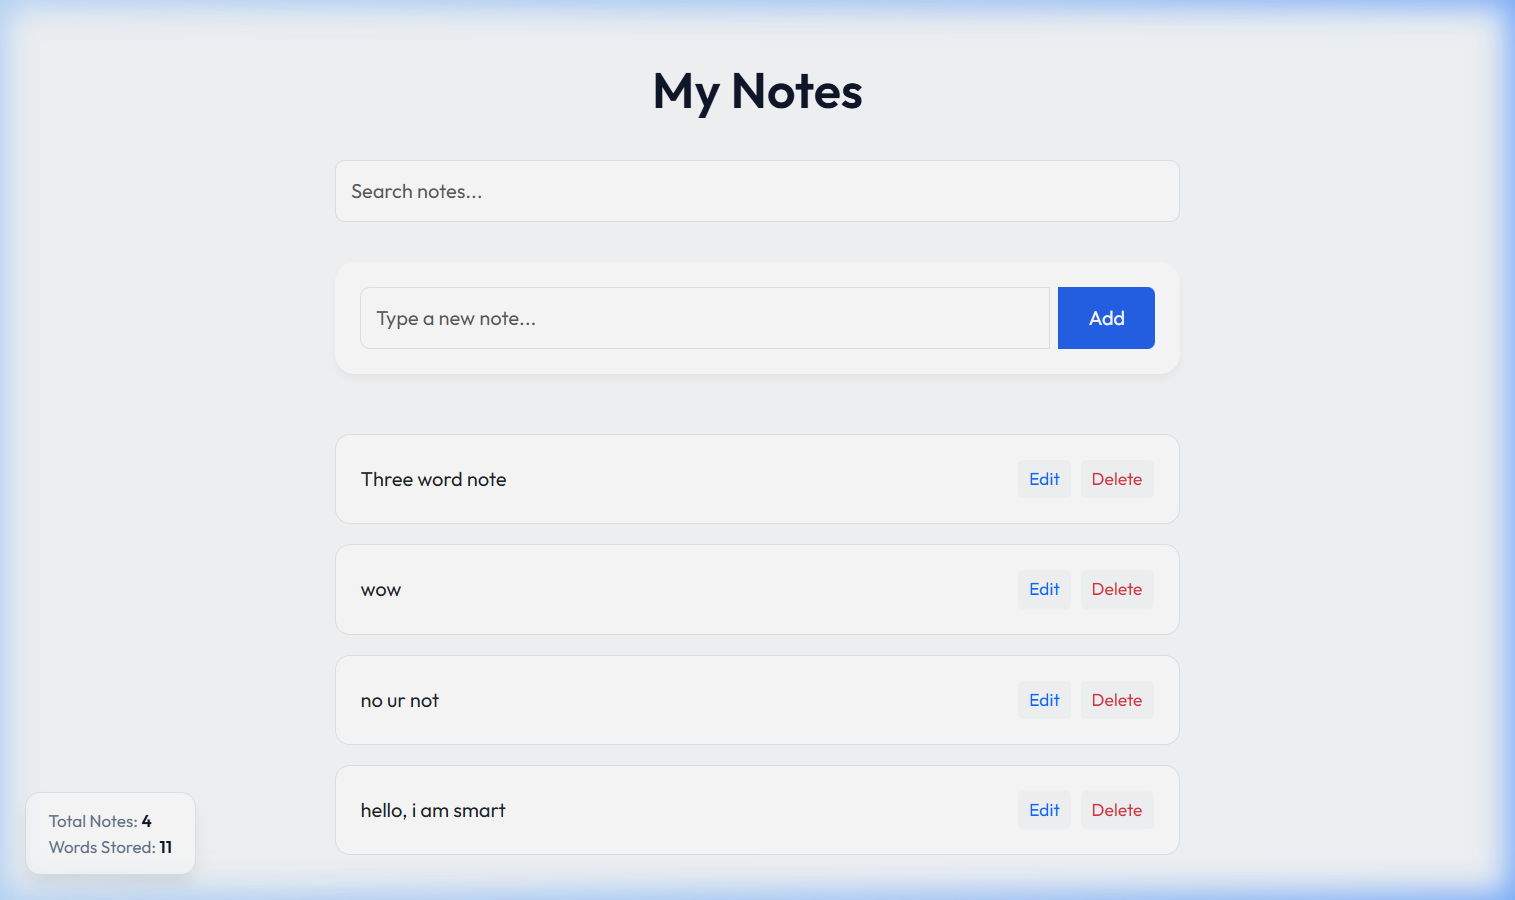
\includegraphics[width=0.3\textwidth]{main_app.png}\\[2cm]
    
    {\large \textbf{SUBMITTED BY:}}\\[0.5cm]
    {\large Atharva Maikhuri (235816206)}\\
    {\large Harshita Gaurav (235816036)}\\[2cm]
    
    {\large April 14, 2026}\\[1cm]
    {\large \textbf{DEPARTMENT OF COMPUTER APPLICATIONS}}
\end{titlepage}

\newpage
\tableofcontents
\newpage

% --- SECTION 1 ---
\section{Project Objective}
The core objective of this project is to develop a lightweight, user-friendly, and highly interactive Note-Taking web application. It serves as a comprehensive demonstration of Full-Stack development concepts, focusing on the seamless integration of a Python-based backend (Django) with a dynamic JavaScript frontend (jQuery \& AJAX).
The application enables users to manage digital thoughts efficiently with zero page reloads, providing a modern Single-Page Application (SPA) experience while adhering to industry standard MVT architecture.

% --- SECTION 2 ---
\section{Technology Stack}
This project utilizes a curated stack designed for performance, modularity, and rapid development.
\begin{itemize}
    \item \textbf{Backend: Django 5.2.13 (Python)}: Chosen for its robust ORM, secure URL routing, and CSRF protection.
    \item \textbf{Frontend: Bootstrap 5 \& Custom CSS}: Provided the grid system and component structure, with custom fade-in animations for a premium feel.
    \item \textbf{Scripting: JavaScript \& jQuery 3.6.0}: Simplified asynchronous communication (AJAX) and real-time DOM manipulation.
    \item \textbf{Database: SQLite}: Used via the Django ORM to provide a zero-configuration, robust storage engine.
\end{itemize}

% --- SECTION 3 ---
\section{System Architecture}
The application follows the Model-View-Template (MVT) design pattern, ensuring a clean separation of concerns.

\begin{figure}[h]
    \centering
    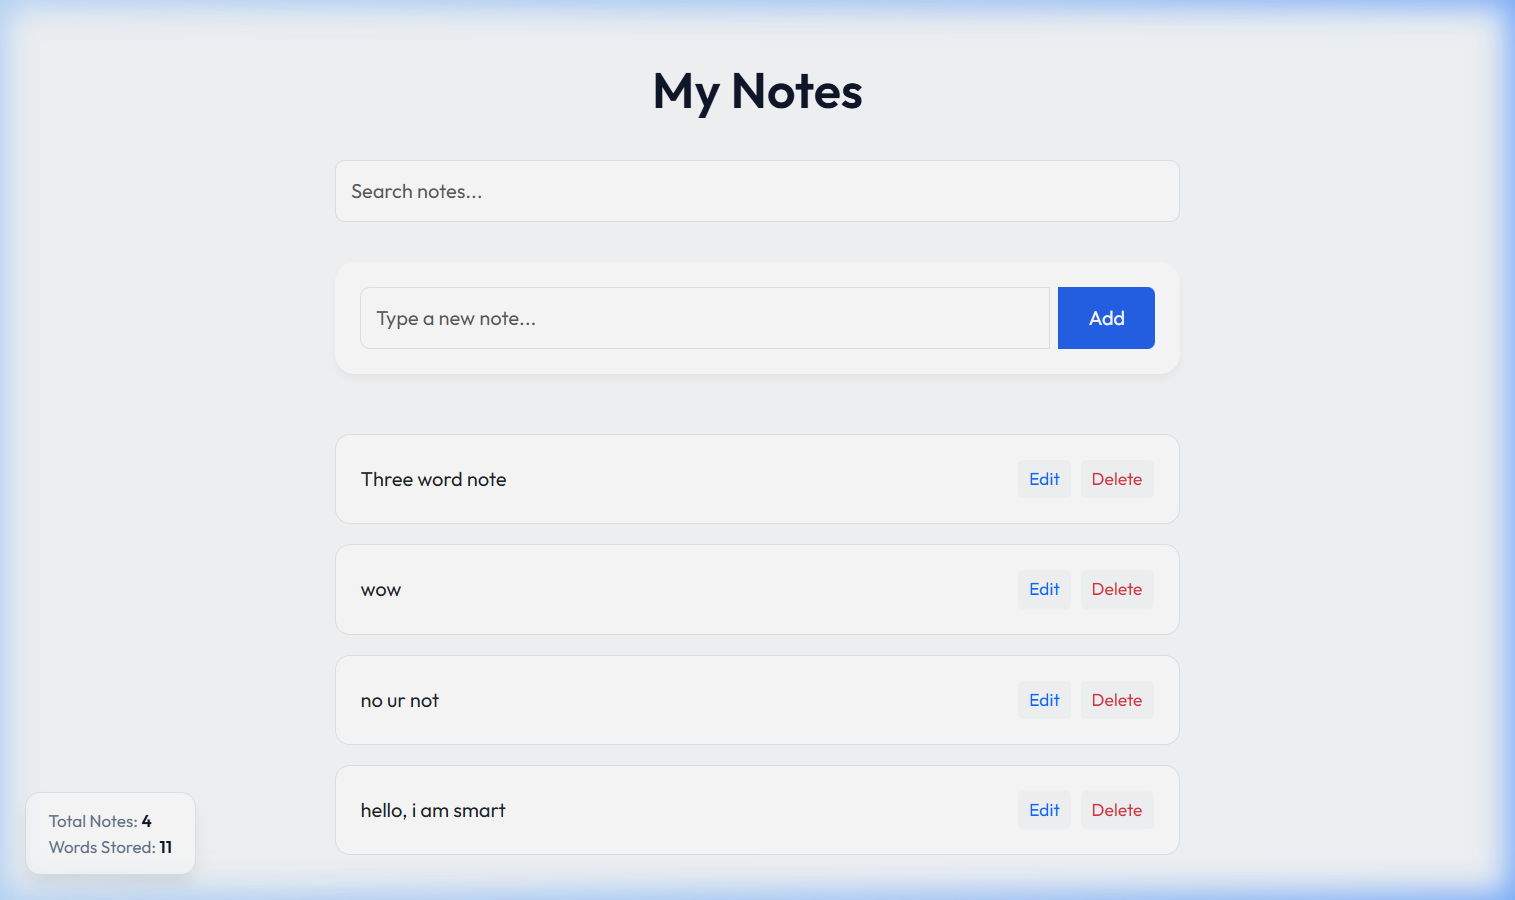
\includegraphics[width=0.8\textwidth]{main_app.png}
    \caption{The Main Dashboard showing live data statistics and the asynchronous notes list.}
\end{figure}

\subsection{System Workflow}
Every user action follows a structured lifecycle:
\begin{enumerate}
    \item \textbf{User Trigger}: User types a note and clicks ``Add''.
    \item \textbf{Asynchronous Intercept}: jQuery prevents the standard form submit and sends a JSON payload via AJAX.
    \item \textbf{Backend Processing}: Django validates the data and creates a record via the ORM.
    \item \textbf{Feedback Loop}: The server returns a success response, and jQuery re-executes the \texttt{loadNotes()} function to refresh the UI.
\end{enumerate}

% --- SECTION 4 ---
\section{Core Features}
\subsection{Live Statistics Tracking}
Calculates and displays real-time statistics (Total Notes, Total Word Count) in the viewport footer.
\subsection{Real-Time Search}
Client-side jQuery filtering for zero-latency feedback during searches.
\subsection{Form Validation}
Blocking empty inputs with high-contrast red feedback (Figure 2.0).
\begin{figure}[h]
    \centering
    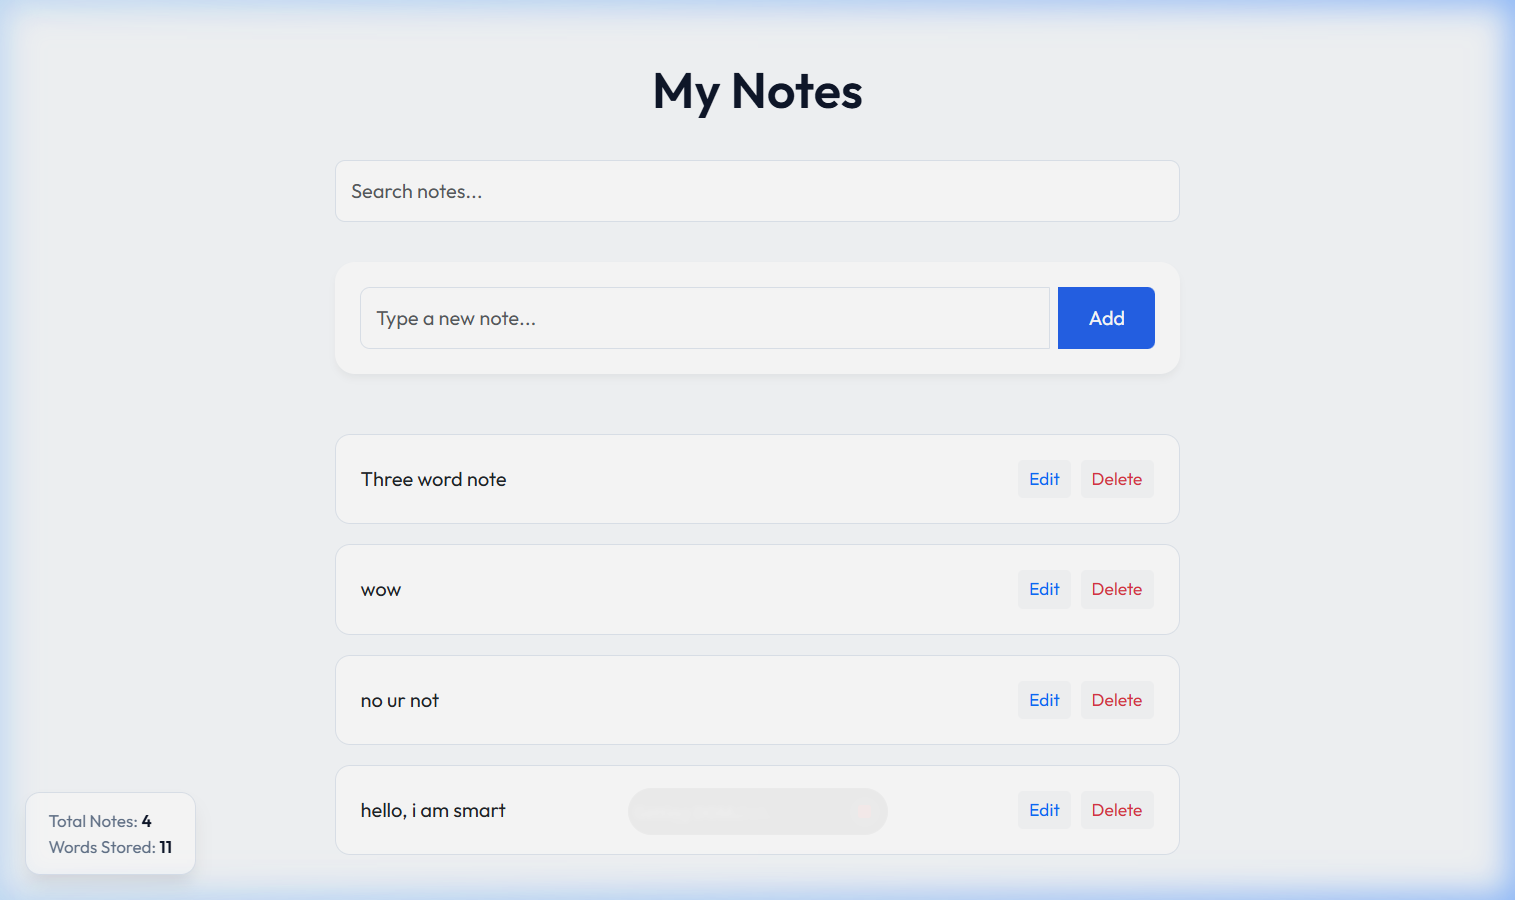
\includegraphics[width=0.6\textwidth]{validation_error.png}
    \caption{Real-time validation blocking empty inputs.}
\end{figure}

% --- SECTION 5 ---
\section{RESTful API Documentation}
The application is built on top of a clean REST API.
\begin{table}[h]
    \centering
    \begin{tabular}{@{}llll@{}}
        \toprule
        \textbf{Method} & \textbf{Endpoint} & \textbf{Payload} & \textbf{Description} \\ \midrule
        GET & /api/notes/ & None & Fetches all notes. \\
        POST & /api/add/ & \{"content": "..."\} & Creates a new note. \\
        POST & /api/update/<id>/ & \{"content": "..."\} & Updates a note. \\
        DELETE & /api/delete/<id>/ & None & Removes a note. \\ \bottomrule
    \end{tabular}
\end{table}

% --- SECTION 6 ---
\section{Interface Design \& Modals}
The app uses an Azure Blue (\#2563eb) theme and centered Bootstrap modals for a focused user experience.
\begin{figure}[h]
    \centering
    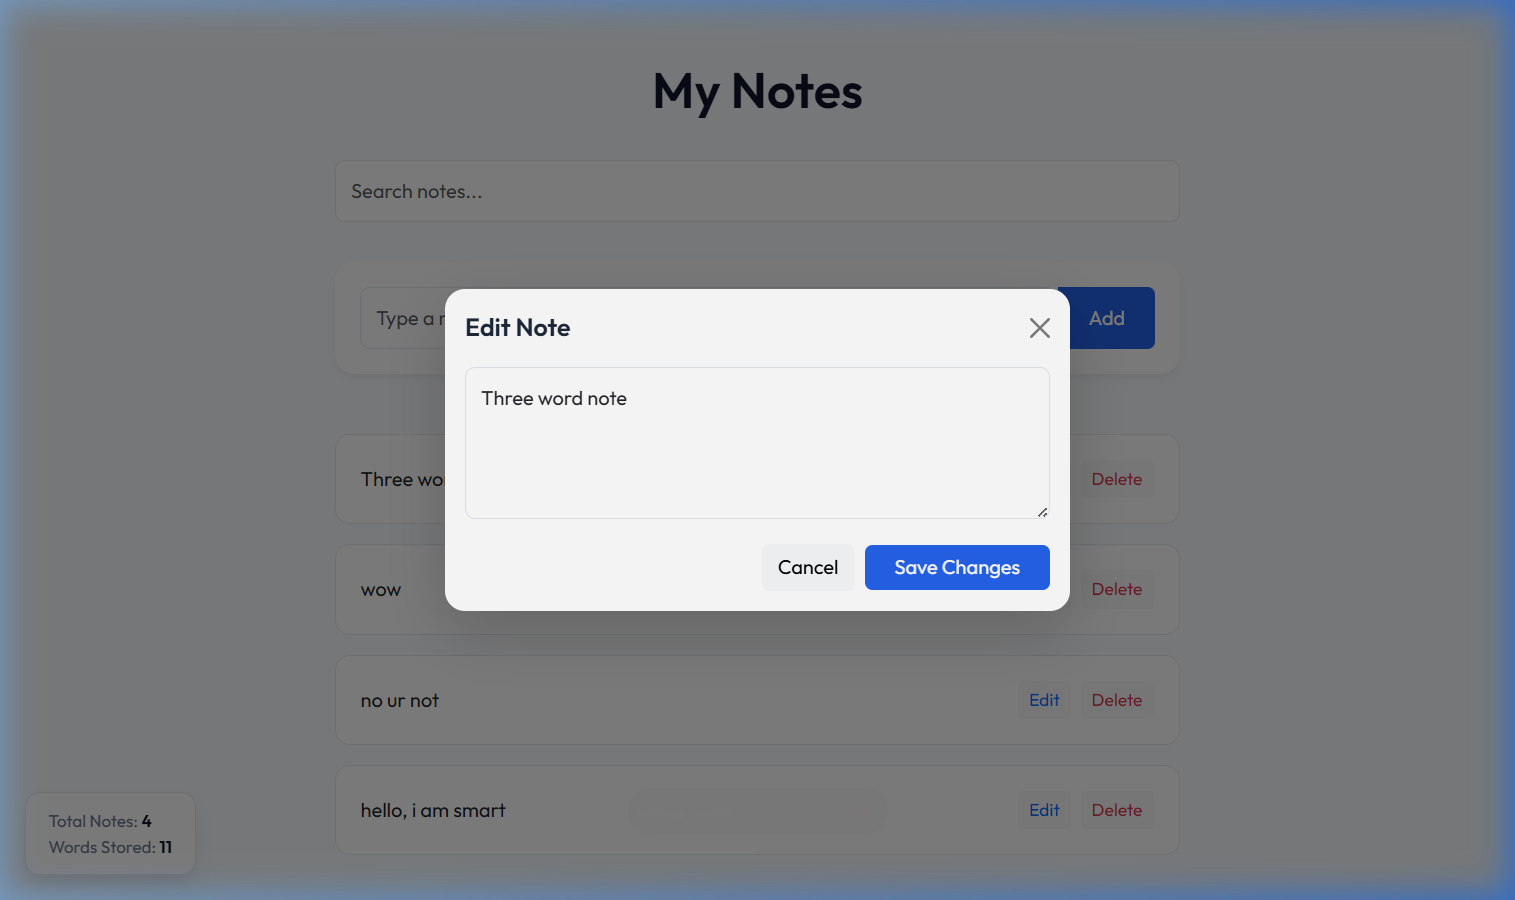
\includegraphics[width=0.6\textwidth]{edit_modal.png}
    \caption{The Edit Modal centered on the viewport.}
\end{figure}

\section{Conclusion}
The Minimalist Notes Application successfully fulfills all requirements of the Lab. By combining a robust Django backend with a dynamic frontend, we created a technically sound and aesthetically pleasing product.

\end{document}
